% This must be in the first 5 lines to tell arXiv to use pdfLaTeX, which is strongly recommended.
\pdfoutput=1
% In particular, the hyperref package requires pdfLaTeX in order to break URLs across lines.

\documentclass[11pt]{article}
\usepackage{graphicx}

\usepackage{float}

% Remove the "review" option to generate the final version.
% \usepackage[review]{acl}
\usepackage{acl}

% Standard package includes
\usepackage{times}
\usepackage{latexsym}

% For proper rendering and hyphenation of words containing Latin characters (including in bib files)
\usepackage[T1]{fontenc}
% For Vietnamese characters
% \usepackage[T5]{fontenc}
% See https://www.latex-project.org/help/documentation/encguide.pdf for other character sets

% This assumes your files are encoded as UTF8
\usepackage[utf8]{inputenc}

% This is not strictly necessary, and may be commented out,
% but it will improve the layout of the manuscript,
% and will typically save some space.
\usepackage{microtype}

% This is also not strictly necessary, and may be commented out.
% However, it will improve the aesthetics of text in
% the typewriter font.
\usepackage{inconsolata}

% INCLUDE additional packages here:
\usepackage{booktabs}

\usepackage{xcolor}
\newcommand{\todo}[1]{\textcolor{orange}{[TODO: #1]}}

% If the title and author information does not fit in the area allocated, uncomment the following
%
%\setlength\titlebox{<dim>}
%
% and set <dim> to something 5cm or larger.
\title{Bridging Feature Spaces: Survey on Multimodal Large Language Model

% Author information can be set in various styles:
% For several authors from the same institution:
% \author{Author 1 \and ... \and Author n \\
%         Address line \\ ... \\ Address line}
% if the names do not fit well on one line use
%         Author 1 \\ {\bf Author 2} \\ ... \\ {\bf Author n} \\
% For authors from different institutions:
% \author{Author 1 \\ Address line \\  ... \\ Address line
%         \And  ... \And
%         Author n \\ Address line \\ ... \\ Address line}
% To start a seperate ``row'' of authors use \AND, as in
% \author{Author 1 \\ Address line \\  ... \\ Address line
%         \AND
%         Author 2 \\ Address line \\ ... \\ Address line \And
%         Author 3 \\ Address line \\ ... \\ Address line}


 \vspace{1em}
  \small{\normalfont WashU CSE527A Survey Paper} }
  
\author{Jianhong Tu \\
  Washington University in St. Louis \\
  \texttt{jianhong.t@wustl.edu} \\\And
  Hongzhang Wang \\
  Washington University in St. Louis \\
  \texttt{hongzhang@wustl.edu} \\\AND
  Alexander Wollam \\
  Washington University in St. Louis \\
  \texttt{atwollam@wustl.edu} \\}

\begin{document}
\maketitle

\begin{abstract}
Large Language Models (LLM) have shown remarkable capabilities in a variety of linguistic tasks, yet their singular modality and inherent limitations have steered research towards Multimodal Large Language Models (MLLM). This survey delves into the core challenges and deficiencies of current LLMs to motivate MLLM research. In our methodology, we dissect strategies for constructing rich multimodal datasets and the interface method of learning a joint representation for vision-language models. We present the performance metrics of prominent models in unimodal and multimodal tasks. Our results shed light on the prowess of MLLMs in transferring useful knowledge across modalities. Despite the promising progress, the current state of MLLMs suffers from imprecise multimodal features and catastrophic forgetting of language abilities.

\end{abstract}

\section{Introduction}
Large language models (LLM) have demonstrated excellent fidelity in high-level tasks, such as multi-step reasoning \citep{DBLP:journals/corr/abs-2112-11446} and instruction following \citep{DBLP:conf/nips/Ouyang0JAWMZASR22}. To enlarge the input space beyond linguistic tokens, researchers proposed multimodal large language models (MLLM) that leverage the idea of \textit{natural language supervision learning} \citep{DBLP:conf/icml/RadfordKHRGASAM21} to annotate features from other modalities with rich and expressive natural language. This survey provides an overview of recent advancements in MLLM and summarises the methods to integrate multiple modalities by unifying information from multiple channels in a general representation space.

\subsection{Multimodality}
"Multimodal" in the context of machine learning refers to models that can process and understand information from multiple types of input \citep{kress2009multimodality}. Although a human's perception of the world is inherently "multimodal," deep learning models, including reinforcement learning, computer vision, and natural language processing, have synchronously evolved in parallel \citep{DBLP:journals/corr/abs-2306-13549}. LLMs that have exploited rich text at a large scale can benefit from the injection of signals from other channels and develop a holistic understanding of real-world concepts.

\subsection{Unimodel Deficiencies}
Pretraining on proxy objectives to acquire general features about the data is a popular DL technique. However, the contribution of each data component often requires ablation studies to be understood since the learned features are highly abstract \citep{DBLP:conf/cvpr/ZhaoJK20}. The expressive natural language has the potential to instantiate abstract signals from images and audio, allowing an intuitive interpretation. In \textit{grounded} tasks that require reasoning with reference to other modalities, especially in robotics, LLMs alone are incapable of reasoning with geo-localization and state estimates in robotic policy \citep{DBLP:conf/icml/DriessXSLCIWTVY23}. Thus, a MLLM tries to complement LLMs with extra information, which is also preferable in human-machine interaction due to its diverse communication flexibility. It renders the model suitable for a wider range of downstream tasks \cite{gpt4, dalle3}.

\subsection{Challenges}
A few unique challenges arise in building an MLLM system. First, abundant textual datasets are crucial to LLM's success, but the availability of large datasets for every modality is not guaranteed. Nevertheless, customized datasets are often needed to supplement existing multimodal datasets, which is hard due to the ambiguity in natural language labels. The pairing of target and ground truth is indefinite since images or other modalities are often open to interpretation. The choice of appropriate representations, or encoders, without compromising any useful signals is also largely experimental. Furthermore, the sub-elements, such as a video frame in a long sequence and its captions, require precise temporal and spatial alignment. Finally, MLLMs need to generalize their understanding to out-of-distribution data instead of "remembering" seen examples. 

\section{Methods}
 To limit the scope, this section focuses on \textit{Vision-Language Models} (VLM) that accepts textual tokens and images and details the methods to construct a joint feature space for the two modalities via step-by-step feature transforming. 

\subsection{Datasets}
Obtaining a large dataset is crucial because the quality of unimodal representation learning is positively proportional to the size of a dataset. Particularly, in learning image representation, the vision transformer, a popular choice in VLM architectures, yields a modest accuracy when trained on a mid-sized dataset but outperforms the SOTA ResNet in image recognition benchmarks after trained on larger datasets \citep{DBLP:conf/iclr/DosovitskiyB0WZ21}. One method to gather sufficient data is to integrate benchmark datasets across domains. The PaLM-E group, concerning robotic policy in addition to visuals and texts, gathered the image captioning data, visual question answer data, text corpus, and robotic navigation data from "SayCan" \citet{DBLP:conf/icml/DriessXSLCIWTVY23}. Appendix A summarizes the common datasets. However, crowd-labeled datasets are often limited in size and serve a general domain. There is a trend to exploit the richness of information from the internet by compiling a customized dataset \citep{DBLP:conf/icml/RadfordKHRGASAM21}. \citet{DBLP:conf/iccv/SunMV0S19} utilized YouTube's audio-transcription to gather 176 hours of synchronous video frames and captions through web API, while \citet{DBLP:conf/icml/RadfordKHRGASAM21} collected approximately 400 million pairs of image and descriptions from public sources. 


\subsection{Joint Representation}
LLMs trained on textual data are incompatible with the raw image data as 3D tensors. A common modeling approach is learning a joint representation of texts, images, and other modalities. Due to the cost of training end-to-end multimodels \citep{DBLP:journals/corr/abs-2306-13549}, it is more feasible to concatenate unimodels pretrained separately into a multimodel. With the LLM as the backbone, a learnable interface projects the image space onto the embedding space \citep{DBLP:journals/corr/abs-2306-13549}, keeping the feature space invariant to pretrained LLMs, thus creating "multimodal sentences." 

Pretraining is a technique to train a task-agnostic model to optimize a proxy objective in order to capture the general features of data. Akin to pretrained embeddings, which can capture semantic similarities, a pretrained ConvNet classifier can encode abstract signals in images such that the hidden layers transform raw images into a feature space where they are linearly separable by a Softmax function and results in 1024-dimensional continuous feature vectors \citep{DBLP:conf/iccv/SunMV0S19}. The continuous features are then tokenized using vector quantization methods to extract $2^{14}$ centroids as the final image representations. Another popular model is the vision transformer, which is an extension of the transformer architecture in CV that can conveniently map images as a sequence of patches into patch embeddings that are inherently compatible with transformer-based LLMs \citep{DBLP:conf/iclr/DosovitskiyB0WZ21, DBLP:conf/icml/DriessXSLCIWTVY23, DBLP:conf/icml/RadfordKHRGASAM21}. The symbolic image representations are appended to the lookup table of LLM as complementary visual vocabulary. 

\subsection{Multimodal Pretraining}
After the LLM is ready to accept multimodal inputs, it is pretrained to establish the connection between image and word embeddings. Most simply, the connection can be learned by treating video embeddings as word embeddings. \citet{DBLP:conf/iccv/SunMV0S19} optimizes a weighted sum of unimodel and multimodel objectives, explained in Appendix B as a training paradigm. More directly, \textit{contrastive objectives} are proposed to fine-tune the text and image encoders by explicitly training on an image-caption pairing task to maximize the cosine-similarity between paired images and text embeddings, which can be understood as minimizing the distance between embeddings with similar semantics \citep{DBLP:conf/icml/RadfordKHRGASAM21}. Another light-weight training scheme, as opposed to the end-to-end training above, is to learn a linking function that transforms images to "prompts" while "freezing" the encoders and the LLM \citep{DBLP:conf/icml/DriessXSLCIWTVY23}. The multimodel is pretrained on next-sentence prediction tasks with sequences of visual and linguistic embeddings, updating the affine transformation function only.

\subsection{Fine-tuning}
\begin{figure*}[t]
    \centering
    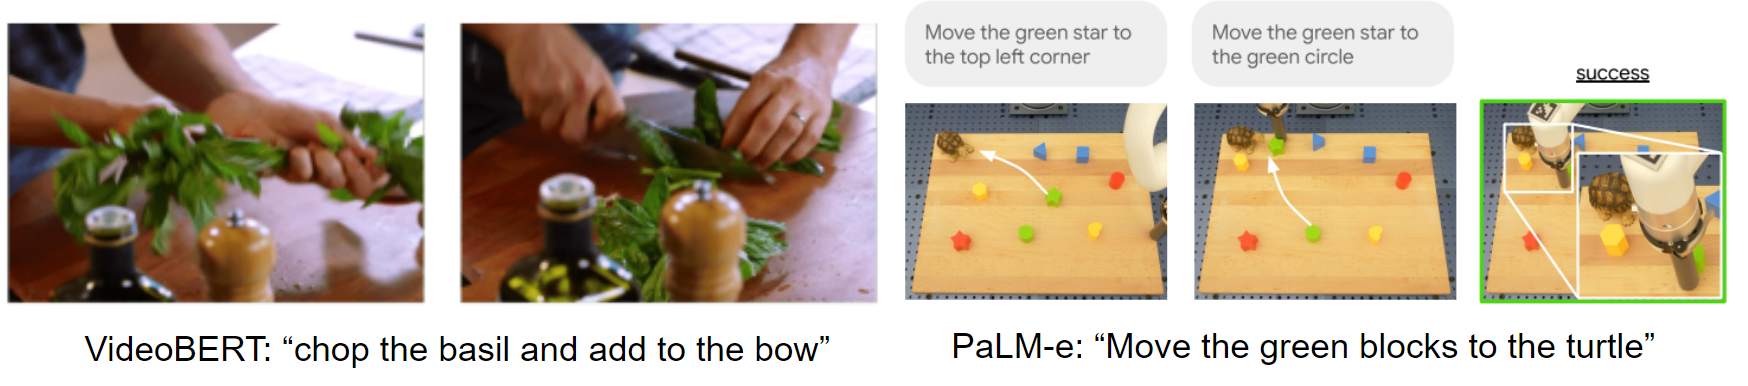
\includegraphics[width=0.80\linewidth]{figures/image.png}
    \caption{Examples of High Level Tasks}
    \label{fig:enter-label}
\end{figure*}
Fine-tuning is a technique to adapt a pretrained model for specific downstream tasks by transferring multimodal knowledge. MLLMs optimize task-specific objectives and are assessed on a curated set of benchmarks, such as VQA \citep{DBLP:journals/corr/abs-2306-13549}. Fine-tuning enables the applications in high-level tasks, which may be evaluated qualitatively. Figure 2 provides 2 examples: VideoBERT model \citep{DBLP:conf/iccv/SunMV0S19} captions the given image by describing the scene and actions and predicting successive steps, while the PaLM-e model \citep{DBLP:conf/icml/DriessXSLCIWTVY23} generates a robotic policy based on the given prompt.

\section{Results}

\subsection{Benchmark scores}
\begin{table}
\scriptsize
\centering
\begin{tabular}{lcccc}
        \toprule
        Model & VQAv2 & & OK-VQA & COCO  \\
        & test-dev & test-std & val & Karpathy test \\
        \midrule
        PaLI-3B & 81.4 & - & 52.4 & 145.4 \\
        PaLI-15B & 82.9 & - & 56.5&  146.2 \\
        PaLI-17B & 84.3 & 84.3 & 64.5 & 149.1\\
        PaLM-E-12B & 77.7 & 77.9 & 60.1 & 136.0 \\
        PaLM-E-66B & - & - & 62.9 & - \\
        PaLM-E-84B & 80.5 & - & 63.3 & 138.0 \\
        \bottomrule
    \end{tabular}
    \caption{Performance of PaLI \citep{DBLP:conf/iclr/Chen0CPPSGGMB0P23} and PaLM-e \citep{DBLP:conf/icml/DriessXSLCIWTVY23} on General Visual-language Benchmarks}
    \label{tab:task_specific_finetuned_models}
\end{table}
\begin{table}[h]
\centering
\scriptsize
\begin{tabular}{c c c c c}
\hline
\textbf{Model} & \textbf{ImageNet} & \textbf{ImageNet-v2} & \textbf{ImageNet-R} & \textbf{ImageNet-A} \\
\hline
PaLI-3B & 70.06 & 62.55 & 80.15 & 37.92 \\

PaLI-15B & 70.27 & 62.81 & 81.21 & 41.16 \\

PaLI-17B & 72.11 & 64.46 & 81.97 & 44.7 \\

CLIP & 76.2 & 70.1 & 88.9 & 77.1 \\

ResNet & 76.2 & 64.3 & 37.7 & 2.7 \\
\hline
\end{tabular}
\caption{Performance of various models on ImageNet benchmarks.}
\label{tab:imagenet_results}
\end{table}
The usage of common benchmarks enables cross-evaluation of different models. Table 1 provides the reference scores of 2 SOTA MLLMs on multimodal tasks. VQA \citep{DBLP:journals/ijcv/GoyalKASBP19} prompts the model to retrieve information from an image and assesses the accuracy. In contrast, COCO caption \citep{DBLP:journals/corr/ChenFLVGDZ15} lets the model generate a description of the image and measures the fluency and consensus with human references via auto metrics like BLUE. Text-only tasks like natural language generation (NLG) are also used to assess whether fine-tuned MLLM retains language ability. Expectedly, frozen MLLM shows no compromise in language ability, though less performant in multimodal tasks. In addition, \textit{zero-shot classification} is of great interest to understand the generalization of abstract knowledge into unseen examples \citep{DBLP:conf/icml/DriessXSLCIWTVY23}. Specifically, researchers studied the transfer of textual knowledge into the CV domain. They assessed the quality of the learned representation by the accuracy of a linear classifier that recognizes objects in images using MLLM as a feature encoder. As presented in Table 2, using Resnet \citep{DBLP:journals/corr/HeZRS15} as the baseline, the features outputted by CLIP \citep{DBLP:conf/iccv/SunMV0S19} and PaLI \cite{DBLP:conf/iclr/Chen0CPPSGGMB0P23} achieves a >70\% accuracy and >40\% accuracy respectively on the most challenging 0-shot classification benchmark "ImageNet-A", versus a mere 2.7\% accuracy for ResNet. In another successive few-shot classification study, CLIP outperforms both ResNet and BiT-M \citep{DBLP:conf/eccv/KolesnikovBZPYG20} and demonstrated better learning efficiency, requiring less data to obtain the same-level performance \citep{DBLP:conf/iccv/SunMV0S19}. Such success suggests a strong co-learning effect; such language abilities help the image knowledge to be more general and robust.

\subsection{Customized Task Performance}
Models fine-tuned to more restricted domains must be assessed using customized benchmarks similar to their training. VideoBERT \citep{DBLP:conf/iccv/SunMV0S19} is evaluated in a task that captions cooking instructional videos. A successful prediction is made when the model generates keywords most relevant to the ground truth caption. MLLM is also applied to the robotics field with the model as the "brain." PaLM-e \citep{DBLP:conf/icml/DriessXSLCIWTVY23} can interact with the environment, which is evaluated on the success rate of carrying out human instruction, i.e., pick up the sponge and then bring it to the user. In a VQA fashion, researchers can assess the model's understanding of the affordance, whether an \textit{action} can be performed on an \textit{entity}. Expectedly, given the same experiment setting, multimodels are reported to outperform the unimodel baseline, meaning a more comprehensive understanding of real-world entities. In general, evaluating customized benchmarks is challenging, and the exact metric is subject to bias.

\section{Discussion}
In the results above, we demonstrate the competitive performance of MLLM models on challenging zero- to few-shot tasks. The high accuracy alludes to the increasing robustness as such generalization entails a successful transfer of knowledge across modalities. However, there is still much room for improvement regarding modality reliability, LLM language capability retention, and efficiency.

\subsection{Modality Reliability}
 Particularly in vision, \citet{fu2023mme} shows that MLLMs can be inconsistent and misidentify sub-elements in images. \citet{DBLP:journals/corr/abs-2306-13549} attributes this issue to information loss due to limited token size capacity, claiming that more efficient image compression is required to break the information bottleneck without worsening the computation burden. Additionally, \citet{fu2023mme} reports that MLLMs tend to hallucinate non-existing features as being present in input images. \citet{DBLP:journals/corr/abs-2306-13549} reasons that this can be ascribed to insufficient modality-alignment pretraining and may be resolved with more fine-grained alignment methods. \citep{DBLP:journals/csur/JiLFYSXIBMF23} describes this behaviour as likely resulting from LLMs' existing tendencies to hallucinate incorrect information—particularly relating to its uncertainty. In summary, the issues stem from both model uncertainty regarding fine-grained features of input images and LLMs' general tendency to hallucinate and respond confidently even when uncertain.

\subsection{Language Capability Retention}
\citet{fu2023mme} demonstrates that MLLMs can fail in instruction following and reasoning, such that these models often do not precisely answer as prompted, and how MLLMs fail to synthesize the key parts into a correct answer. Both of these shortcomings are surprising since LLMs generally accomplish them well. \citet{DBLP:conf/icml/DriessXSLCIWTVY23} offer an analysis of these pertinent issues by directly contrasting the performance of their foundational PaLM with its multimodal variant, PaLM-E, across various model scales in the context of Natural Language Generation (NLG) tasks. They show that the smaller models trained on the multimodal objectives face catastrophic forgetting and perform significantly worse. This issue is alleviated for their largest model, where performance only drops a few percent, suggesting the importance of scale to MLLM. The lackluster language capability retention relates to MLLMs forgetting much of their text-only pretraining when optimized end-to-end; this may be mitigated by simultaneous training on multimodal and text-only NLG objectives without increasing model complexity.

\subsection{Future Work}
Both issues above can be alleviated through sheer model scale—allowing for more precise representations of images and more intact language abilities. Though the ever-increasing size is the key recipe to LLM's success, it is of even greater importance for MLLMs due to the need to capture more complex multimodal relations at the unfortunate cost of efficiency. Since a full suite of pretraining and end-to-end optimization is also needed to reach the full potential of MLLMs \citep{DBLP:conf/icml/DriessXSLCIWTVY23}, advanced data compression techniques and parameter-efficient training is of great concern to reduce load.

\section{Conclusion}
This survey presented a general overview of recent MLLMs. We first motivate these models by introducing the restrictions of LLMs due to incompatibility to modalities other than language, which limits their application in a wider range of real-world scenarios, as well as the challenging task of bridging the multimodal space. To learn potent joint representations, we present the SOTA methods to collect sufficient training datasets and to adapt other modalities into pretrained LLMs through a learnable interface. We then illustrate the robust performance in both multimodal and unimodal tasks thanks to the transfer effect as well as the unfortunately degraded language abilities. Finally, this survey addresses the issue of information bottleneck that requires a more efficient training scheme and better information compression techniques in future research.

% Entries for the entire Anthology, followed by custom entries
\bibliography{anthology,custom}
\newpage

\appendix

\section{Example MLLM Datasets}

\begin{table}[H]
    \centering
    \small
    \begin{tabular}{l|l|l|l|}
        \hline
        Dataset & Task & Size \\
        \hline
        TAMP & Robotic manipulation planning with VQA & 96000 scenes & Source\\
        Language Table & Robotic manipulation planning & 600000 sequences & \citet{DBLP:conf/icml/DriessXSLCIWTVY23}\\
        Mobile Manipulation & Robotic navigation and manipulation planning with VQA & 2912 sequences of action & \citet{DBLP:conf/icml/DriessXSLCIWTVY23}\\
        VQA2v & Question answering with images and prompts & 1.1M questions with images &\citet{DBLP:journals/ijcv/GoyalKASBP19}\\
        COCO & Image captioning & 123287 images with captions & \citet{DBLP:journals/corr/ChenFLVGDZ15}\\
        OK-VQA & Visual question answering requiring external knowledge & 14031 questions with images &\citet{DBLP:conf/cvpr/MarinoRFM19}\\
        YouCook & Instructional video captioning & 2000 videos with caption & \citet{DBLP:conf/iccv/SunMV0S19}\\
        CLIP benchmark & Image captioning & 400M image-text pairs & \citet{DBLP:conf/icml/RadfordKHRGASAM21}\\
        \hline
    \end{tabular}
    \caption{Summary of MLLP datasets}
    \onecolumn
\end{table}

\twocolumn
\section{Multimodal BERT Objectives}
\label{sec:appendix}
Pretraining of a multimodel is commonly conducted in a step-by-step fashion: first, the encoders of various modalities are trained, then the pretrained models are concatenated into a multimodel and pretrained on visual-linguistic tasks to acquire a general embedding space of visuals and texts. Here, we explain the pretraining objectives of VideoBERT \citep{DBLP:conf/iccv/SunMV0S19} as a paradigm of multimodel pretraining. 

VideoBERT is a masked multimodal large language model. With the images summarised into $2^{14}$ discrete tokens, both word embeddings and image tokens can be accepted as input to the BERT model, as a multimodal sentence. As far as VideoBERT is concerned, the visual input is a sequence of down sampled video frames that has inherent temporal alignment similar to sentences. We may view it as a "visual sentence" of image tokens. For each modality, the sequences of words or video frames are randomly masked so the model is trained to restore the maksed embeddings, which is termed masked-prediction objective. The video-only training objective is thus analogous to the text-only or the Valina BERT training objective. It helps the model to acquire long-term state dependencies in video frames. Formally, training each modality separately ensures the model's capability to capture the marginal distribution of image $P(x)$ or text $P(y)$.

The third training objective establishes the joint distribution $P(x,y)$ so that the model understands the interplay of video and texts. To encode image information into sequences of word embeddings, word-based sentences, and visual tokens are combined into visual sentences joined by a special token "[>]."
\begin{verbatim}
    [CLS] orange chicken with [MASK] sauce 
    [>] v01 [MASK] v08 v72 [SEP]
\end{verbatim}
Researchers proposed a \textit{linguistic-visual alignment} task, where the state of the "[cls]" token is used to determine whether the linguistic sequence and the visual sequence are aligned, which is, to some degree, similar to the \textit{next-sentence prediction} task in the vanilla BERT model. This objective essentially establishes the connection between the two domains. 

After pretraining, the model would learn a joint representation of multi-modalities. Further fine-tuning allows it to be used in various downstream tasks.


\end{document}
